\chapter{Likovno upodabljanje slik}\label{chp:LikovnoUpodabljanjeSlik}
%
Likovno upodabljanje slik (v nadaljevanju LUS) je področje v računalniški grafiki, ki se ukvarja z vprašanjem kako realistični medij slike pretvoriti v artistično likovno delo. V nasprotju z realističnim upodabljanjem, kjer je poudarek na podrobnostih, pri LUS poskušamo upodobiti imanentne informacije. LUS ima zelo široko uporabo pri upodabljanju slik, risb, tehničnih ilustracij, risanih animacij itd. V nasprotju s fotorealističnimi slikami imajo tako dobljena likovna dela namreč to prednost, da lahko likovni umetnik (ali tehnični risar) da poudarek na določen detajl slike, omeji količino podrobnosti, prilagodi paleto barv ali npr.\ doda sliki svojo osebno noto.

LUS se je razvilo iz računalniškega področja prepoznavanja (geometrijskih) oblik na sliki in digitalne obdelave slik. Z razvojem filtrov za obdelavo slik, ki so sprva služili bolj kot npr.~orodje pri tehnični obdelavi medicinskih slik, se je sčasoma njihova uporaba razširila tudi v umetniške vode. Prišlo je do razvoja računalniškega poustvarjanja določenih li\-kov\-ni\-h stilov, kjer so izkoristili lastnosti in delovanje filtrov. 

V prvem razdelku si bomo najprej pogledali primer uporabe filtrov za dosego nekega likovnega efekta na dani fotografiji. Ugotovili bomo, da uporaba filtrov, ki delujejo lokalno, ne pripelje do kompleksnih artističnih efektov. V preostalih razdelkih bomo zato spoznali različne načine za likovno upodabljanje slik, kjer se bomo poslužili modelov čopiča, svinčnika in voščenke ter med drugim uporabljali tudi optimizacijski pristop za slikanje in ustvarjanje mozaikov. V vsakem razdelku bomo navedli nekaj osnovnih člankov in njihovih povzetkov, na podlagi katerih si lahko bralec ustvari predstavo o bogatem dogajanju na področju LUS.
%%
%%
%%
\section{Artistični filter}\label{sec:ArtisticniFilter}
%
Obstaja tudi vrsta komercialnih programov, ki ustvarjajo slike s pomočjo artističnih filtrov, npr.\ Adobe Photoshop.
%%
%%
%%
\section{Tehnične ilustracije}
%
\emph{Tehnična ilustracija} je

\begin{figure}[htb]
  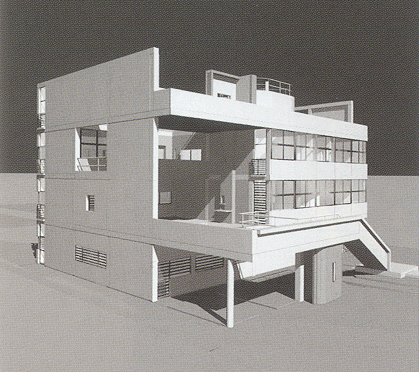
\includegraphics[width=0.49\textwidth]{./slike/real.png}
  \ \ 
  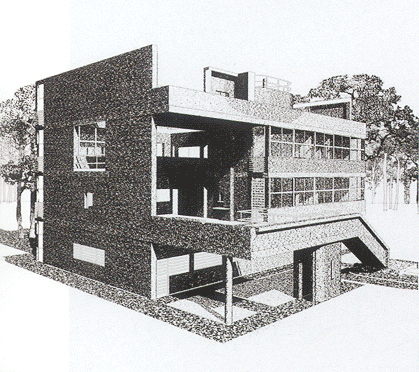
\includegraphics[width=0.49\textwidth]{./slike/npr.png}
  \caption{Razlika med realističnim upodabljanjem in likovnim upodabljanjem.}
\end{figure}
 
Leta 1991 sta Seligmann in Feiner v \cite{Seligmann:Automated} opisala metodo za avtomatično konstruiranje 3D %BAUER Ali je 3D v matematičnem načinu 
ilustracij. Ustvarjanje ilustracij poteka znotraj sistema stilističnih pravil in tehničnih zahtev, ki določajo končni videz ilustracije in jih lahko izbere uporabnik programa. Njun sistem Njihov osnovni cilj je high-level of compositing the best model for comunicatting a particular intent. Yessios je opisal prototip sistema za upodabljanje materialov v arhitekturnih načrtih, kot so kamni, les, rože in tla. Namesto mehaničnega videza želijo ilustracijo prikazati z nežnejšimi potezami. % TODO nežnejšimi ;)
Miyata \cite{Miyata:Stone} je opisal algoritem za upodabljanje vzorcev kamnitih sten. Appel je z soavtorji v \cite{Appel:Haloed} predstavil metodo, s katero narišemo črto, ki ima videz, da gre zadaj za drugo. Kamada in Kawai \cite{Kamada:Hidden} sta posplošila nuno delo in ppredstavila različne parametre črte, kot so črtkanost, pikčastost, \ldots, s pomočjo katerih lahko skrite črte vizualno boljše predstavimo. Dooley in Cohen sta kasneje v \cite{Dooley:Lines, Dooley:Surfaces}  predstavila še več parametrov linij, kot je npr.\ debelina črte in podala diskusijo o načinu uporabnikove interakcije, da bi izboljašlai likovni vtis ilustracij, pri čemer bi obravnavali obliko objekta (linije, ki ga določajo) in njegovo senčenje.

Saito in Takahashi sta v \cite{Saito:3Dshapes} predstavila koncept $G$-bufferja %TODO prevod za G-buffer
za ustvarjanje razumljivih upodobitev 3D scen. Njihova metoda v bistvu po tem, ko ustvarijo množico $G$-bufferjev, uporablja tehnike iz procesiranja slik. V \cite{Wikenbach:ComputerGenerated} sta Winkenbach in Salesin opisala tradicionalne pristope za upodabljanje slik na pen-and-ink način in pokazala, da lahko mnoge izmed njih implementiramo kot del avtomatskega likovnega upodabljanja slik. Predstavila sta stroke texture, % TODO prevedi stroke texture
s pomočjo katerega lahko tako teksturo kot tudi senčenje dosežemo z risanjem linij. Stroke texture dovoljuje tudi likovno upodabljanje slik, ki je odvisno od izbrane resolucije. Opisane tehnike sta demonstrirala s pomočjo kompleksnega arhitekturnega modela, ki vključuje tudi Lloyd's Wright's Robie House. Svoje delo sta v \cite{Winkenbach:ParametricSurfaces} nadgradila, kjer sta uvedla nove algoritme in tehnike za likovno upodabljanje parametrično podanih površin, ki imajo nepravilno obliko. Predstavila sta idejo hatchinga, % TODO hatching - prevod
kjer kontroliramo gostoto risanja linij, da bi dosegli želejeni ton senčenja, obliko in teksturo. Pokazala sta tudi kako lahko ravninski zemljevid, %TODO graf ?
ki je glavna podatkovna struktura pri njunem upodabljanju ilustracij, konstruiramo iz parametrično podanih površin in ga uporabimo za rezanje linij in ustvarjanje linij, ki omejuje objekte. Za ukrivljene objekte sta predstavila tudi senčenje, ki posnema linijo ukrivljenega objekta, ki ga upodabljamo.

Lansdown in Schofield sta v \cite{Lansdown:Expressive} sta predstavila sistem Piranesi, ki uporablja tehnike likovnega upodabljanja za ustvarjanje ilustracij iz podanega 3D modela. Piranedsi uporablja standarne grafične plinovode, % TODO daj link; pipeline
s pomočjo katerih ustvari 2D reliefno sliko. Uporabnik lahko nato posameznim območjim na sliki določi teksturo ali pa je ta določena avtomatsko.

Salisbury je skupaj s sodelavci v \cite{Salisbury:OrientableTextures} predstavil interaktivni sistem za risanje ilustracij na podlagi črnobele vhodne slike, kjer linije na ilustraciji posnemajo obliko objektov na vhodni sliki. Uporabnik, preko novih tehnik za dodajanje vektorskega polja, določi orientacijo za vsako posamezno območje. Računalnik nariše linije, ki temeljijo na uporabnikovih primerih liniji in poskusi doseči iste tone na ilustracji kot so na vhodni sliki, s pomočjo novega algoritma, ki primerja zamegljeno verzijo trenutne ilustracije z vhodno sliko. S poravnanim vektorskim poljem z orientacijami površin objektov na sliki lahko uporabnik ustvari teksturo, ki ima videz, da je pritisnjena na površino, namesto da z njo le potemnimo neketere dele. To ima kot posledico bolj privlačne ilustracije, kot smo jih lahko poprej upodobili iz 2D slik.

Goodwin \cite{Goodwin:IsophoteDistance} s sodelavcama je predstavil pristop za določanje debeline črt v računalniško generiranih ilustracijah gladkih površin. Predpostavka, da se poudarjene črte rišejo na tistih območjih slike kjer je temnejše senčenje, jih je vodila do preproste formule za debelino linij, ki omejujejo objekte in tistih linij, ki sugestirajo detajle na objektih. Formula je odvisna od globine, ukrivljenosti in smeri svetlobe. Za upodabljanje linij uporabijo lokalno obliko in relacijo globine.

\section{Risbe}
Risbe so med osnovnimi likovnimii komunikacijami, ki človeku pomagajo v možganih reproducirati vhodno sliko risbe. Risanje s svinčnikom lahko razdelimo v dve skupini glede na vhodne podatke. te lahko namreč dobimo kot 2D informacijo ali pa kot 3D model. Glavna likovna stila, ki ju s svinčnikom poskušamo upodobiti sta skica ()%TODO povej kaj je skica
in hatching (z risanjem na istem mestu v enakih ali različnih smereh poskušamo doseči določeni ton slike). % TODO prevode
Sousa in Buchanan \cite{Sousa:Model} sta predstavili modele za grafit, papir za risanje, radirke. S temi modeli predstavi  teksturo, ton in %TODO popravi
Modeli so narejeni na podlagi interakcije med grafitom svinčnika in papirja ter na podlagi lastnosti radiranja in smoofanja % TODO kaj je to smufanje ?
S pomočjo parametrov, kot je %TODO iz članka povzetek \cite{Sousa:Polygonal} in \cite{Sousa:Blenders} iz članka ven unga lepega

Lee s sodelavci so v \cite{Lee:RealTime} iz podane 3D površine objekta izločili linije, ki objekt omejujejo in jih predelali za simulacijo ročno narisanih linij. Senčenje simulirajo s pomočjo teksture svinčnika in pa usmerjenih linij. Temelji na svetlobi in materijalu danega 3D modela. Pri upodabljanju slik s svinčnikom so algoritmi najpogosteje taki, da dobijo za vhodni podatek 3D model in nato poskušajo dobiti informacijo o linijah za risbo iz modela \cite{DeCarlo:Photographs, Judd:Ridges, Lee:Abstracted, Grabli:Programmable}. Rusinkiewicz je v \cite{Rusinkiewicz:Review} naredil pregled likovnega upodabljanja s svinčnikom na podlagi danega 3D modela.

V \cite{Lake:Stylized} je bil predstavljen model senčenja. Različne hatching stile sta definirala Hertzmann in Zorin v \cite{Hertzmann:Illustrating}. Praun pa je skupaj sodelavci \cite{Praun:ReaTime} razvil algoritem za hatching, ki se izvaja v realnem času. V \cite{Chen:Example} je predstavljen algoritem za risanje potretov s svinčnikom s stilom, ki posnema določeno tradicijo ali pa stil risarjev.

Mao s sodelavci v \cite{Mao:Automatic} so predstavili postopek za lokalno strukturo orientacije na podlagi vhodne slike in vključili linearno integracijsko konvolucijo (LIC) z namenom simulacije efekta senčenja. Yamamoto pa je s sodelavci v \cite{Yamamoto:Filter} je razdelil vhodno sliko na plasti z različnimi toni v različnih obsegih. Li in Huang \cite{Li:Feature} sta uporabila geometrijske parametre, from ... % TODO lepi članek poglavje 2
%
% TODO kod bodo mozaiki omenjeni
\section{Painterly rendering}
Cohen \cite{Cohen:Aaron, Morbey:Aaron} se je problema risanja oz.\ slikanja lotil z vidika umetne inteligence. Ustvaril je sistem Aaron, ki na podlagi množice randomiziranih pravil ustvari originalno kompozicijo v določenem artističnem stilu. Aaron ima na voljo tudi robotsko slikanje.
  
Haeberli je v \cite{Haeberli:PaintNumbers} predstavil interaktivni sistem za slikanje, ki ustvari impresionistično sliko iz fotografije. Poteze čopiča je upodobil v vrstnem redu. Vsaka poteza je imela parametre (položaj, barva, velikost in oblika), ki so bili večinoma določeni interaktivno, tj.\ s pomočjo uporabnika. Shiraishi in Yamaguchi \cite{Shiraishi:LocalSource} določata orientacijo in obliko potez čopiča na podlagi lokalnih značilnosti vhodne slike. Curtis in ostali avtorji so v \cite{Curtis:Watercolor} predstavili semi-avtomatski algoritem za upodabljanje watercolor slik. %TODO prevod za watercolor
Njihov algoritem ne bo ustvaril vidnih potez čopiča, zato s tem izgubijo artistični vtis slikanja s čopičem. Litwinowicz \cite{Litwinowicz:VideoImpressionist} je opisal avtomatičen sistem za postavitev potez čopiča na podlagi vektorskega polja izračunanega iz gradienta vhodne slike in uporabil rezanje potez na robovih slike. Izhodna slika algoritma je naslikana v impresionističnem stilu, za katerega so značilne kratke poteze. %TODO kam vtaknit to, da je impresionistično
Sistem je razširil na likovno upodabljanje posnetkov. Za upodabljanje posnetkov je uporabil kratke poteze in premikal narisane poteze na platnu s pomočjo izračunanega optičnega toka, ustvarjenega na podlagi posnetka. Pristop, ki ga je Litwinowicz uporabil za postavljanje potez na platno (tj.\ postavitev potez na mrežo) je najbolj pogost način, ki ga uporabljajo za upodabljanje slik s čopičem. Razlike med algoritmi so v obliki in orientaciji potez. Treavett in Chen \cite{Treavett:Statistical} sta predstavila način za likovno upodabljanje s statistično analizo vhodne slike, na podlagi katere določita položaj, orientacijo in velikost upodobljenih potez. Litwinowicz in Treavett s Chenom so sliko pobarvali enoplastno. Pri enoplastnem slikanju je potrebno natančno predviditi položaje in obliko potez, kar pa je težaven problem. Pomankljivost takih algoritmov je torej v tem, da ne moremo morebitnih detajlov in napakic, ki nastanejo pri slikanju ne moremo naknadno popraviti še z eno plastjo potez čopiča. Hertzmann je v \cite{Hertzmann:BrushStrokes} predlagal način upodabljanja slik z večplastnim slikanjem, kjer postavlja na platno poteze čopiča različnih debelin in oblik, ki jih določi s pomočjo Bezierovih krivulj. Začetno točko poteze ne postavi na mrežo slike, temveč v okolici mrežnih točk poišče točko z največjo napako. Kontrolne točke Bezierovih krivulj pa poišče na podlagi izračunanega gradienta vhodne slike. Tak način upodabljanja slikanja je tudi najbolj podobno dejanskemu načinu slikanja. Slikar namreč najprej naredi grobo sliko, ki jo nato z manjšimi čopiči popravi na delih, kjer je potrebno več poudarka in detajlov. S pomočjo te metode lahko ustvarimo sliko, ki ima artistični vtis, vendar pa je potratna in detajlov na sliki vedno ne nariše lepo. To metodo je Hertzmann skupaj s Perlinom razširil na upodabljanje posnetkov \cite{Hertzmann:Video}.

Ročno narisane poteze s čopičem nimajo konstantne barve vzdolž poteze, temveč imajo vgrajeno strukturo. Običajna metoda za upodobljanje potez čopiča je s pomočjo antialiazirane črte, ki ima konststno barvo. Litwinowicz je v \cite{Litwinowicz:VideoImpressionist} predstavil idejo dodajanja teksture in svetlobe pri upodabljanju potez. Hertzmann je v \cite{Hertzmann:Texture} predstavil posebno tehniko za dodajanje efekta svetljenja za likovno upodobljene slike s pomočjo višinskega polja slike in bump-mappinga. %TODO to morš lepo napisat
V \cite{Huang:Natural} so Huang in sodelavci predstavili podoben način kot je bump-mapping, vendar je bistveno enostavnejši za implementacijo. Predstavili so model anizotropičnega čopiča. Upodobaljanje potez poteka tako, da pripravljeno masko čopiča (na podlagi ...)%TODO napiši še kaj

Hays in Essa sta v \cite{Hays:Animation} predstavila uniform %TODO uniform kot kaj
likovno upodabljanje za slike in posnetke. Za razliko od večine prejšnjih algoritmov, so poteze pri tej metodi postavljene na večjem platnu. Orientacije za poteze so izračunane z RBF interpolacijo. Pri upodabljanju posnetkov, se parametri potez med postopkom spreminjajo, orientacija potez pa je določena z vektorskim poljem na podlagi gradienta posameznih sličic, različne frekvence robov na sliki pa pripomorejo h upodobitvi detajlov na sliki.

%TODO manjka še tazadni del, pa pejd po novem članku

Uporaba informacije o 3D geometrijski strukturi slike, ki jo želimo likovno upodobiti, nam dovoljuje veliko več fleksibilnosti pri ustvarjanju posnetkov. Meier iz Walt Disney Feature Animation je %TODO povej da je Disney
v \cite{Meier:Animation} predstavila avtomatičen sistem, ki postavlja poteze čopiča na podlagi opisa posameznih delov slike. %TODO preberi kaj naredi
V filmih \textit{Tarzan} \cite{Daniels:Tarzan} in \textit{What Dreams May Come} %TODO daj imbd linke
so bile uporabljene razširitve tega algoritma.  Tak sistem naravno zagotavlja časovno koherenco in ekonomičnost likovnega upodabljanja posnetka. Vendar pa podatki o geometrijski strukturi niso vedno dosegljivi. Klein \cite{Klein:Virtual} je objekte upodobil s pomočjo filtrirane strukture. % TODO poglej si
Uporaba 3D strukture tipično proizvede drugačen srtistični učinek, saj so poteze čopiča vezane na geometrijsko struktuo objektov. Turk in Banks sta v \cite{Turk:Guided} za ilustriranje vektorskega polja z uporabila relaksacijo. Njuno delo in uporabo relaksacije, ki jo je uporabil Haeberli v \cite{Haeberli:PaintNumbers}, je Hertzmann razširil v članku \cite{Hertzmann:Relaxation}.

Lee je v \cite{Lee:Motion} predstavil novo metodo za za določanje oprientacije potez čopiča v likovnem upodabljanju posnetkov. Informacijo o premikih, ki jo dobimo iz zaporedja sličič posnetka uporabimo za orientiranje potez čopiča v območjih, kjer je bilo zaznano večje gibanje. %TODO v uvodu splošnem že povej, da so pri upodabljanjih videjov problem šum
V območjih z rahlio zaznanim gibanjem pa določimo orientacijo potez čopiča na podlagi gradienta slike. % TODO I guess
Določanje orientacije po tem postopku ima prednost pri izražanju gibanja objektov. 